\documentclass[12pt]{article}
\usepackage{sbc-template}
\usepackage{graphicx}
\usepackage{url}
\usepackage[brazil]{babel}
\usepackage[utf8]{inputenc}
\usepackage{paralist}
\usepackage{listingsutf8}
\usepackage{amssymb}
\usepackage{amsmath}
\usepackage{subfigure}

\sloppy

\title{Simulando movimento de bando de passáros em JavaScript}

\author{Guilherme Henrique Polo Gonçalves}

\address{Departamento de Informática\\
  Universidade Estadual de Maringá (UEM) -- Maringá, PR -- Brasil
  \email{ggpolo@gmail.com}
}

\begin{document}

\maketitle

%\begin{abstract}
%Empty abstract.
%\end{abstract}

%\begin{resumo}
%Resumo vazio.
%\end{resumo}


\section{Introdução}
A simulação do movimento em bando praticado na natureza, Figura
\ref{fig:nature}, foi desenvolvida para simplificar e tornar
mais real a forma como é feita a animação de elementos que
descrevem movimentos complexos.

\begin{figure}[h!]
  \centering
  \subfigure[Na natureza (foto de Tim Edelsten)\label{fig:nature}]{
    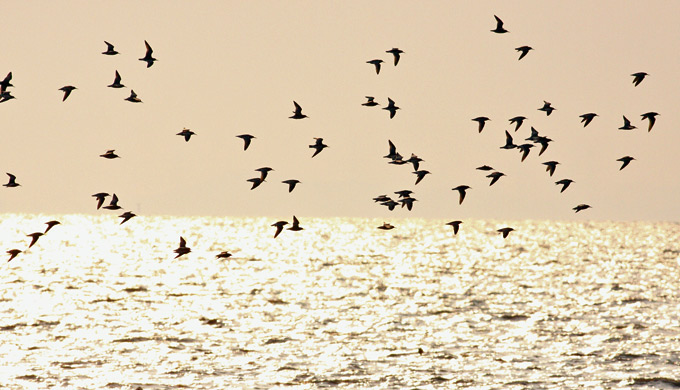
\includegraphics[width=7cm]{figs/knot_flock.jpg}
  }
  \subfigure[Em filme \label{fig:lionking}]{
    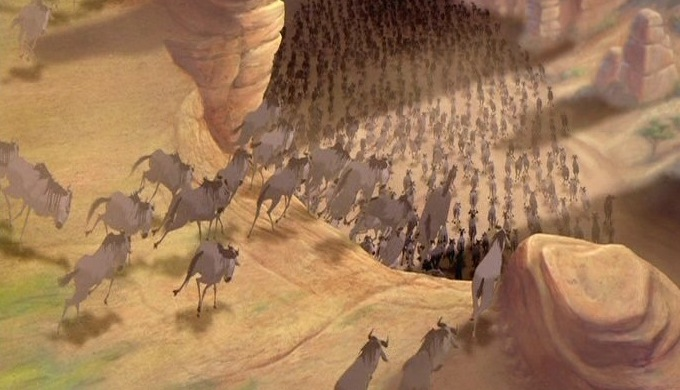
\includegraphics[width=7cm]{figs/lionking_wide.jpg}
  }
  \caption{Ocorrência de bandos}
\end{figure}

O trabalho de \cite{reynolds} descreveu uma abordagem para essa
simulação, tendo como foco os pássaros. Simular um bando de pássaros,
nesta abordagem, equivale a simular o comportamento individual de cada
pássaro. Entretanto, o comportamento individual inclui a percepção
necessária para coordenar o voo e indiretamente criar um
bando. Este modelo de simulação tem sido adaptado e utilizado em cenas
de filmes, como aquela do Rei Leão onde ocorre a debandada de gnus,
Figura \ref{fig:lionking}. No presente trabalho seguiu-se os conceitos
introduzidos por Reynolds, que são apresentados agora.

Um pássaro simulado é denominado de \textit{boid}, que vem de
\textit{bird-oid} (pássaróide -- uma mistura de pássaro com andróide),
e obedece a três regras:

\begin{enumerate}
\item Evitar colisão com pássaros próximos;

\item Esforçar-se para manter uma aceleração próxima daqueles
  ao seu redor;

\item Tentar ficar suficientemente próximo de outros pássaros para manter
  o bando.
\end{enumerate}

A proximidade entre dois \textit{boids} é, geralmente, dada pela
distância e direção de deslocamento. Definir um ponto onde dois
pássaros passam a estar próximos é específico da implementação. A
aceleração é um vetor formado pela combinação entre direção de
deslocamento e velocidade atual.

Além destas regras que descrevem o comportamento de um bando, o artigo
de \cite{reynolds2} apresenta outras que servem para complementar a
simulação. Duas delas foram utilizadas
aqui: \begin{inparaenum}[(1)] \item Evitar colisão com objetos; \item
  Vagar pelo mundo\end{inparaenum}. A primeira destas é utilizada pois
o mundo simulado pode conter obstáculos; a segunda é aplicada, neste
trabalho, a um \textit{boid} quando o mesmo estiver fora de um bando.

Para desenvolver esta simulação, a linguagem de programação
\texttt{JavaScript} \cite{jsref} foi utilizada por apresentar boa
portabilidade e atualmente estar presente em grande parte dos
\textit{browsers}. A seção seguinte descreve o que foi desenvolvido e
em seguida alguns experimentos sobre esta implementação são
apresentados.


\section{Implementação}

O aplicativo desenvolvido simula o comportamento do movimento em bando
em duas dimensões e trata os indivíduos como pontos. Essas
especificações simplificam a implementação, não sendo necessário
tratar deslocamento e rotação no eixo z além de reduzir a quantidade de
cálculos necessários para a aplicação das regras. A Figura
\ref{screen1} apresenta uma visão geral do aplicativo em execução.

\begin{figure}[ht!]
  \centering
  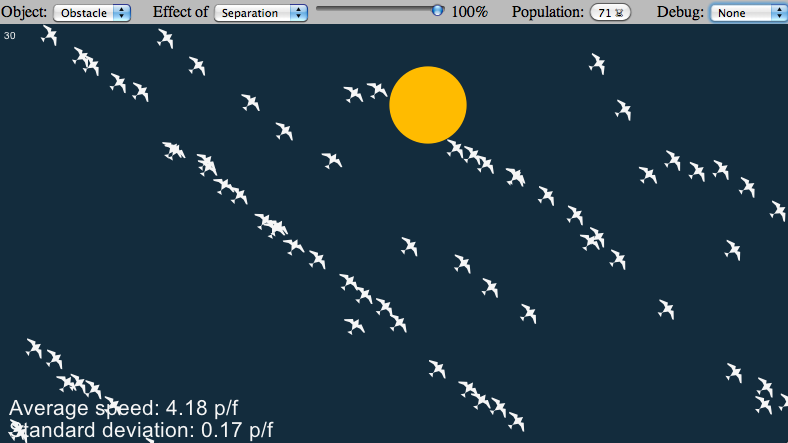
\includegraphics[height=8cm]{figs/screen1.png}
  \caption{Aplicação em execução com 71 pássaros e um obstáculo em amarelo \label{screen1}}
\end{figure}

No topo da Figura \ref{screen1} estão contidos os controles
disponíveis ao usuário. Pode-se criar obstáculos ou pássaros
selecionando o respectivo objeto por meio de um menu (aquele mais a
esquerda) e clicando em qualquer posição do grande retângulo azul
escuro. O efeito de cada regra sobre cada pássaro pode ser ajustado no
controle logo a direita deste primeiro. Para matar um \textit{boid}
pode-se clicar no botão que apresenta o tamanho da população atual
seguido de uma caveira. %{\fontspec{Symbola}☠}.
Por último, é possível exibir informações
a respeito da visão dos \textit{boids} ao alterar o nível de depuração
exibido.

O ângulo de visão de cada \textit{boid} é utilizado para a aplicação
das três regras descritas por Reynolds. Num primeiro momento
considerou-se uma visão de 360$^o$, simplificando a detecção de
\textit{boids} vizinhos. Entretanto, optou-se por tratar o ângulo de
visão como um parâmetro de modo a permitir testes sobre o
mesmo. Atualmente este ângulo é fixado em 270$^o$, onde tal número foi
obtido do estudo realizado em \cite{birds} que indica um campo de
visão de 135$^o$ em cada olho para um tipo específico de
pássaro. Este valor é dito ser fixo por razão do aplicativo não
disponibilizar um controle sobre o mesmo para o usuário. %, mas tal
%ângulo pode ser facilmente modificado no código.
Também é considerado
um raio para a aplicação das regras 2 (alinhamento) e 3 (coesão) e um
outro raio para a regra 1 (separação). Escolheu-se dois raios
distintos por considerar que a separação só é necessária quando
\textit{boids} estão muito próximos, ao passo em que manter um bando
requer um maior número de informações ao redor de cada
\textit{boid}. A Figura \ref{screen2} apresenta estas informações mencionadas.

\begin{figure}[ht!]
  \centering
  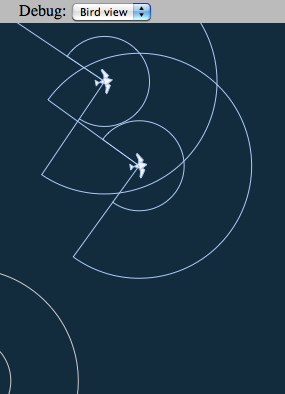
\includegraphics[height=8cm]{figs/birdview.png}
  \caption{Visão dos \textit{boids} \label{screen2}}
\end{figure}

Na Figura \ref{screen2}, o setor circular interno representa a região de
separação enquanto que o externo descreve aquela onde as outras duas
regras para bandos aplicam-se. Nota-se que há um setor circular parcial,
na parte inferior à esquerda da figura, com cor cinza, indicando que o
pássaro ali presente não esta em um bando e, portanto, vaga pelo mundo.

A implementação das regras de separação, alinhamento e coesão foi
feita seguindo o artigo de \cite{reynolds2}. A primeira destas obtém
um vetor que
corresponde a média da soma das distâncias entre o \textit{boid} em
consideração e os demais em seu raio de separação, levando em conta
que uma distância maior representa uma necessidade menor de
separação. A regra de alinhamento consiste em realizar uma média das
direções de deslocamento daqueles \textit{boids} contidos no raio
maior do \textit{boid} em consideração. Na coesão é feito uma média
das posições atuais dos \textit{boids} existentes no raio maior,
efetivamente indicando uma posição de centro de massa para onde um
\textit{boid} específico deverá ser deslocado. Em todas as regras
têm-se um vetor resultante que são somados e que indicam como cada
pássaro deve responder ao ambiente. Entretanto, para tornar esta
resposta menos artificial, os movimentos são limitados de forma que
não ocorram movimentos bruscos entre um \textit{frame} e outro. Atualmente, os
vetores são limitados ao comprimento 0,065 (valor arbitrário, obtido
por experimento) e resulta em movimento mais suaves.

Os últimos pontos a serem tratados dizem respeito a detecção de
colisão. Há duas formas de colisão: \begin{inparaenum}[(1)] \item
  entre \textit{boids}; \item entre
\textit{boid} e obstáculo\end{inparaenum}. Neste segundo caso é feito
uso de um retângulo, Figura \ref{screen3}, que estende-se além do
raio de aplicação de outras regras.

\begin{figure}[ht!]
  \centering
  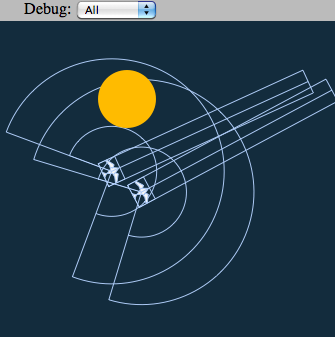
\includegraphics[height=8cm]{figs/avoidobst.png}
  \caption{Retângulo para detecção futura de colisão com obstáculos \label{screen3}}
\end{figure}

Nos dois casos de detecção de colisão realiza-se uma translação,
considerando a posição do \textit{boid} corrente como origem, e uma
rotação considerando a direção de deslocamento do mesmo. Ao aplicar estas
operações, torna-se mais simples detectar a colisão. Para o caso de
retângulo e círculo (\textit{boid} e obstáculo), verifica-se se o centro,
na coordenada x,
do obstáculo encontra-se na frente (a direita) do pássaro e se a
distância até esta coordenada é menor que o comprimento do retângulo mais o
raio do círculo. Satisfazendo estas condições, verifica-se se
$|P_y| < C_r + \frac{R_A}{2}$, com $P_y$ representando a coordenada y
do centro do 
círculo, depois de transladada e rotacionada, $C_r$ equivalendo ao
raio do círculo e $R_A$ sendo a altura do retângulo. Para determinar a direção de deslocamento de forma a
desviar do obstáculo, escolhe-se o vetor normal em relação a direção de
deslocamento atual com base no ponto de colisão com o círculo de modo
que seja necessário menor esforço por parte do \textit{boid} para
desviar com sucesso. O outro caso de colisão, ponto com setor circular
(\textit{boid} e \textit{boid}), é tratado de forma similar. A
diferença é que após realizar a translação e rotação, aplica-se a
função arco tangente no ponto resultante para identificar se o
respectivo ângulo encontra-se na faixa $\pm$ 135$^o$.


\section{Experimentos}

Dois experimentos foram realizados: \begin{inparaenum}[(1)]
\item determinação do tamanho de população com desempenho
  perceptivelmente ruim; \item aplicação isolada da regra de
  separação\end{inparaenum}.

Para replicação mais próxima do primeiro experimento deve-se
considerar os seguintes requisitos: sistema operacional Mac OS X
10.6.5; processador Intel Core 2 Duo, modelo P8700; memória principal
de 4 GB de 1066 Mhz, PC3-8500 DDR3 SO-DIMM SDRAM; \textit{browser}
Safari 5.0.3. Este experimento verificou que uma
população inicial de tamanho superior a 130 causa uma perceptível
demora no ínicio, sendo este um dos momentos de maior intensidade
computacional pois todos os \textit{boids} foram
criados num mesmo ponto e, portanto, há uma grande quantidade de vizinhos
a serem considerados na aplicação de regras. Ao longo da simulação,
aumentou-se a população até 250 e então notou-se baixo desempenho:
taxa de atualização abaixo de 30 quadros por segundo (topo esquerdo da
Figura \ref{screen1}) com visível degradação do movimento suave. Isso
indica que a implementação realizada tem baixo desempenho, visto que
apresenta custo computacional $O(n^2)$
para aplicação das regras a cada \textit{frame}. Para simular
populações maiores, uma alternativa seria trabalhar com métodos de
implementação mais eficientes \cite{maisefici1}\cite{maisefici2} para
simulação de bandos.

No segundo experimento foram verificadas quais diferenças surgem durante a
simulação no caso de aplicar a regra de separação de forma
exclusiva. Ou seja, caso um \textit{boid} precise realizar a separação
então esta é a única regra aplicada. Inicialmente sempre combinou-se
as três regras para movimento em bando, mas ao pensar que um pássaro
nunca irá desejar colidir com outro torna-se interessante
visualizar o que isto causa na simulação. A Figura \ref{screen4}
apresenta as diferentes formações durante a inicialização da simulação
e a Figura \ref{screen5} exibe o resultado obtido num estado mais
estável. Ambas simulações utilizaram o mesmo \textit{seed}.

\begin{figure}[h!]
  \centering
  \subfigure[Inicialização, regras não exclusivas]{
    
\includegraphics[height=5cm]{figs/start1_nonex.png}
  }
  \subfigure[Após inicialização, regras não exclusivas]{
    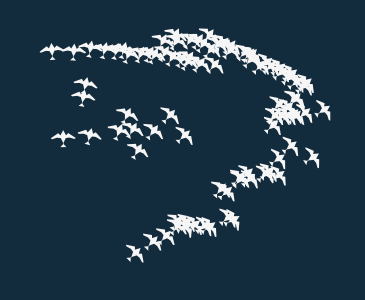
\includegraphics[height=5cm]{figs/start2_nonex.png}
  }
  \subfigure[Inicialização, separação exclusiva]{
    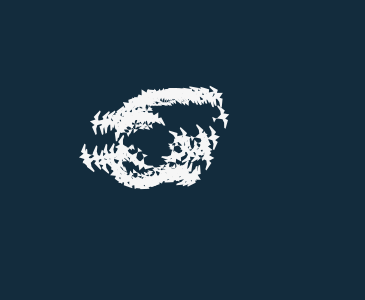
\includegraphics[height=5cm]{figs/start1_ex.png}
  }
  \subfigure[Após inicialização, separação exclusiva]{
    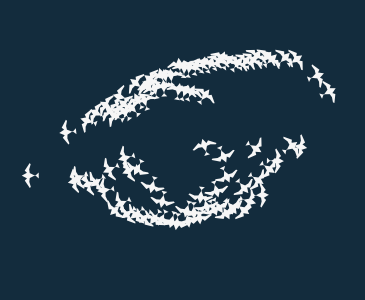
\includegraphics[height=5cm]{figs/start2_ex.png}
  }
  \caption{Fase mais intensa de aplicação de regras \label{screen4}}
\end{figure}

Na Figura \ref{screen4} nota-se que com uso de regras não exclusivas a
tendência é a formação de um único bando logo no ínicio. Por outro
lado, aplicar a regra de separação de forma exclusiva causa um maior
espalhamento dos \textit{boids} e cria-se mais de um bando neste momento.

\begin{figure}[h!]
  \centering
  \subfigure[Regras não exclusivas \label{nonexc}]{
    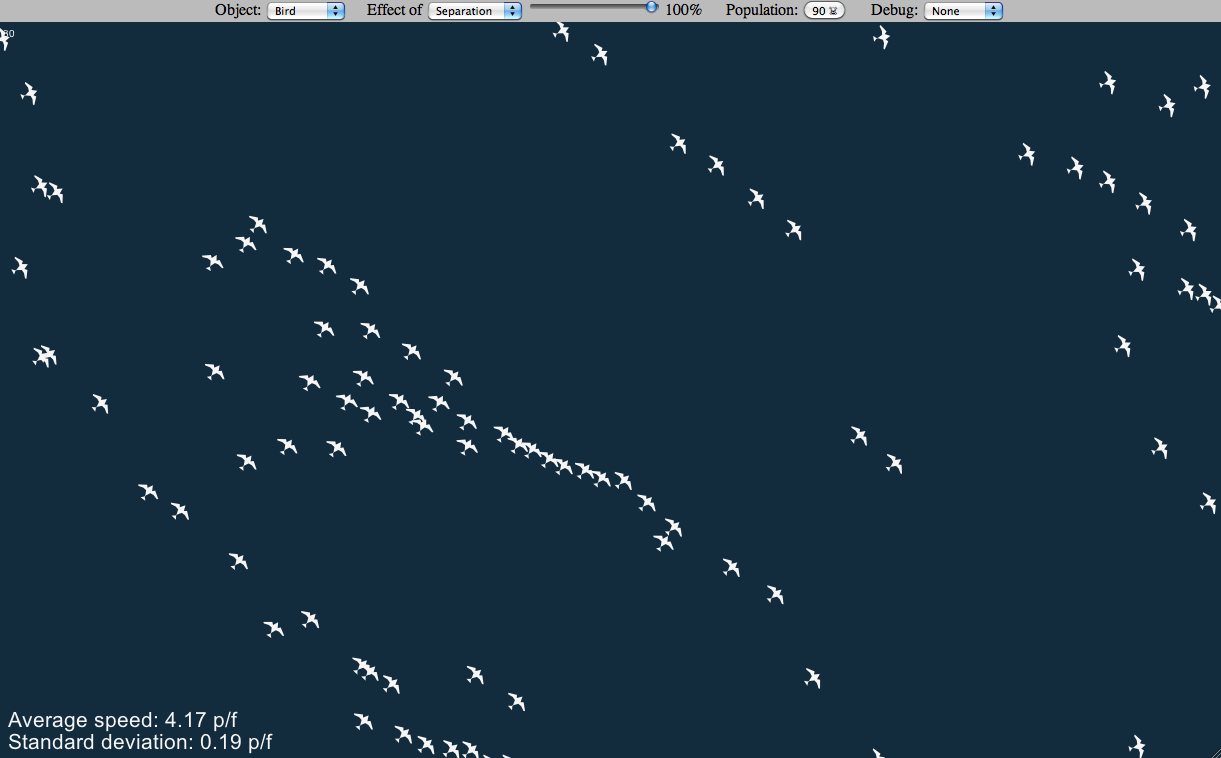
\includegraphics[height=7cm]{figs/steady_nonex.png}
  }
  \subfigure[Separação exclusiva \label{excend}]{
    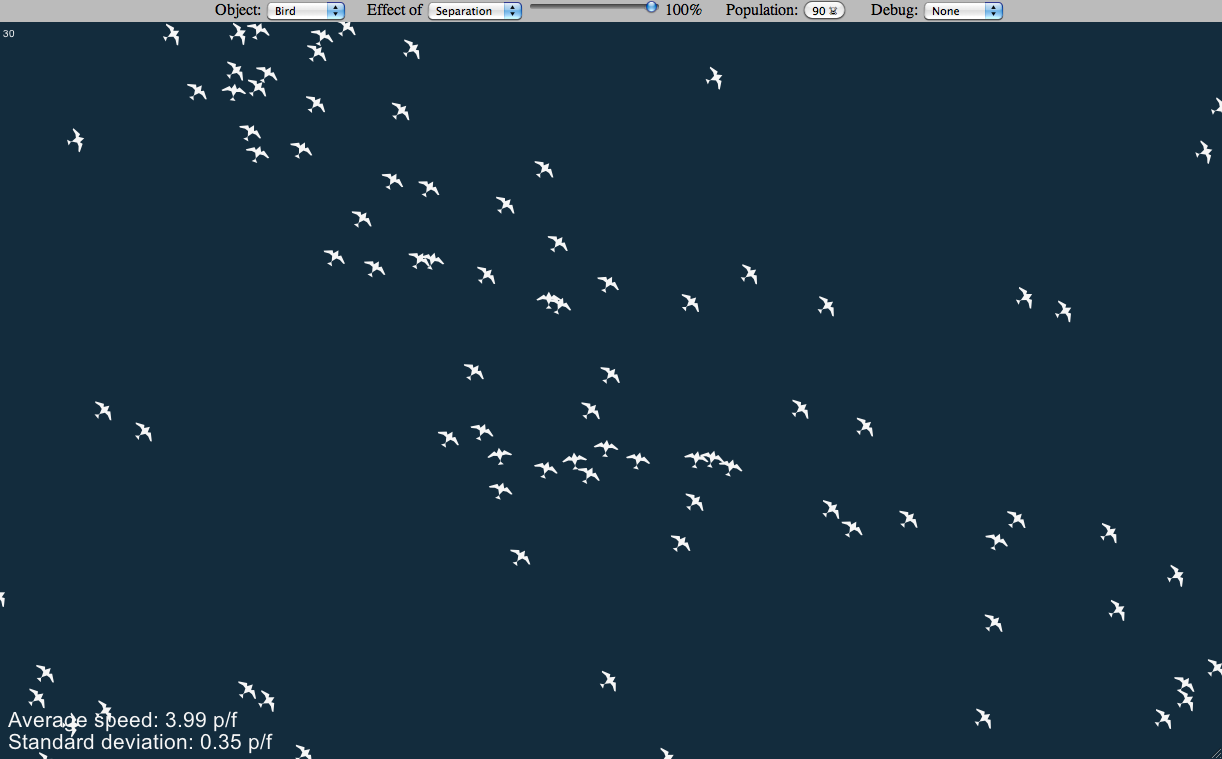
\includegraphics[height=7cm]{figs/steady_ex.png}
  }
  \caption{Estado quase estável da simulação \label{screen5}}
\end{figure}

A Figura \ref{screen5} conclui o experimento. Nestes casos
ocorreu que a observação inicial se manteve ao longo da
simulação. Ou seja, a tendência de manter um único bando ou quase todos
\textit{boids} em bando (mesmo que em diferente bandos) permaneceu com
o uso de regras não exclusivas. Pode-se notar uma formação mais caótica
na Figura \ref{excend}, enquanto que no outro caso (Figura
\ref{nonexc}) a direção dos
pássaros aparenta maior uniformidade. O fato
dos \textit{boids} estarem em bando em maior quantidade na
Figura \ref{nonexc} também é indicado pelo desvio padrão da velocidade
média calculada em $\frac{pixels}{frame}$, com este estando mais
próximo de 4,2 p/f, que é o valor atingido por bandos nesta simulação.
%Entretanto, saber quais das duas situações ocorre na natureza com
%maior frequência, ou qual das duas esta menos distante da realidade,
%não é respondido neste trabalho.
Pela aparente maior tendência a formação de bandos, na implementação
final optou-se por manter regras não exclusivas.

Um outro experimento a ser feito diz respeito a força
aplicada sobre cada regra. No momento, os valores iniciais foram
arbitrariamente escolhidos como 100\%,
70\% e 75\% para as regras de separação, alinhamento e coesão,
respectivamente. Talvez outros valores, juntamente com a utilização de
ângulo de visão variável, podem vir a causar efeitos distintos, como a
formação em V.


% Referências
\bibliographystyle{sbc}
\bibliography{biblio}

\end{document}
